\subsection{Introduktion}


Administrationssystemet er en applikation som kan tilføje, fjerne og redigere produkter eller kategorier i  systemets produktkatalog.\\
Applikationen er designet skalerbart, således brugeren ikke er begrænset til kun at kunne tilføje, fjerne eller redigere fra udelukkende en node, men derimod synkront holde databasen opdateret fra flere noder på en gang. Dette betyder at produktkataloget og alle opkoblede administrationssystemer, altid vil være helt synkroniseret.

\subsubsection{Design og struktur}
Backend er designet på baggrund af MVVM designmønstret~\cite{MVVM}. 

\begin{figure}[!h]
    \centering
    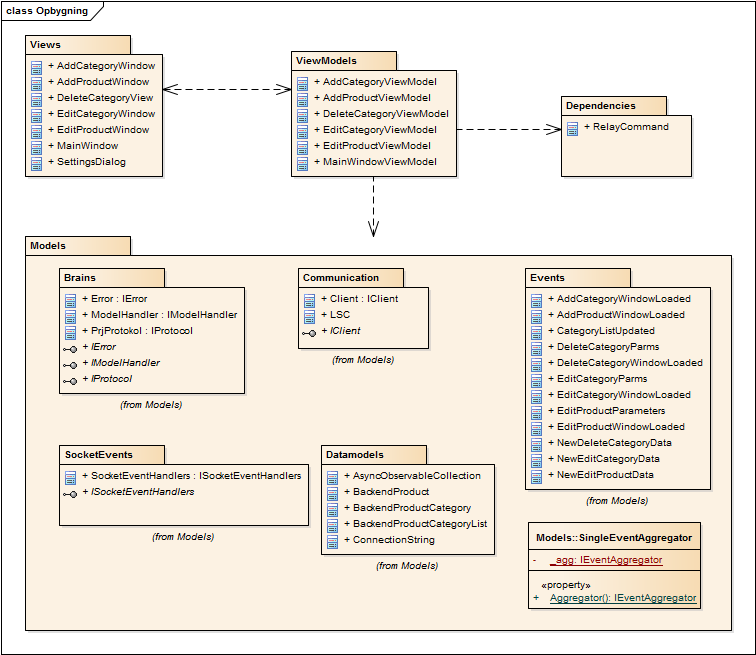
\includegraphics[width=1\textwidth]{Systemdesign/backend/Images/Opbygning.png}
    \caption{Oversigt over alle namespaces i administrationssystemet}
    \label{fig:oversigtAs}
\end{figure}

På figur \ref{fig:oversigtAs} ses det hvordan strukturen i administrationssystemet er opbygget. MVVM er valgt som overordnet design, således at presentation logic og business logic holdes adskildt. Desuden giver MVVM er godt overblik, og gør systemet skalerbart. Eksempelvis kunne ny funktionalitet, eksempelvis et lagervindue, tilføjes nemt ved at lave et view, viewmodel og det logik der nu skal til, \textit{uden} at det påvirker noget af det eksisterende.\\\\

Herunder ses en kort beskrivelse af de forskellige namespaces, og hvad de indeholder.

\begin{itemize}
\item \textbf{Views} indeholder XAML og codebehindfilerne for den grafiske brugerflade. 
\item \textbf{ViewModels} indeholder de data og commands som views binder til. 
\item \textbf{Models} indeholder datamodeller og business logic.
\item \textbf{Datamodels} indeholder datamodeller, herunder bl.a. produkter, collections og kategorier.
\item \textbf{Events} indeholder events der bruges til kommunikation mellem viewmodels, den tilhørende aggregator samt parametermodellen\footnote{Tit kaldet EventArgs i C\#} til nogen af disse events.
\item \textbf{SocketEvents} indeholder de events der bliver raised af Client ved modtagelse af data.
\item \textbf{Brains} indeholder generel businesslogik til bl.a. at oprette kommandoer til klienten og fejl-håndtering.
\item \textbf{Dependencies} indeholder sourcekode, RelayCommand~\cite{RelayC} til at arbejde med commands mere effektivt.
\item \textbf{Communication} indeholder klient til at skabe forbindelse til Central Server.
\end{itemize}

Det er valgt at dele så meget op i namespaces som muligt, således at overblikket kommer hurtigt, også selvom man ikke kender systemet. 
